\chapter{Feasibility study} \sloppy
\hbadness=99999 
\section{Technical Feasibility} 
For the technical part, we obtained our project data from the IStego100K\cite{7} dataset, which contained 200,000 images. These images had been modified using three different algorithms, which created diversity in the dataset used, improving the reliability of the system. We used free software to build the project, and for the training and testing, we used our own computers. Thus, we concluded that it was technically feasible.

\section{Economical Feasibility}
The only cost for the project is the computational power, covering processing and electricity.
For development of the system, all the softwares used are free of cost and hardwares
were available for us to train model.

\section{Operational Feasibility}
We had decided to use the Shallow ML approach, which allowed the model to be trained with less computational power in comparison to deep learning. For shallow machine learning, we planned to implement an ensemble classifier, and each of its models was trained using FLD to improve its effectiveness. Deep learning implemented the CNN approach, which required higher computational power to be trained. Thus, we decided to use a simpler machine learning approach that didn't need a lot of computational power, unlike the more complex deep learning method called Convolutional Neural Network (CNN). This way, the system was practical and didn't need a lot of resources, making it able to be effectively implemented in real-life applications, making it operationally feasible.

\section{Schedule feasibility} 
The project was scheduled to be completed within in 6 months duration. Our project completed as scheduled in Gantt chart.

\section{Gantt Chart}
\begin{figure}[H]
    \centering
    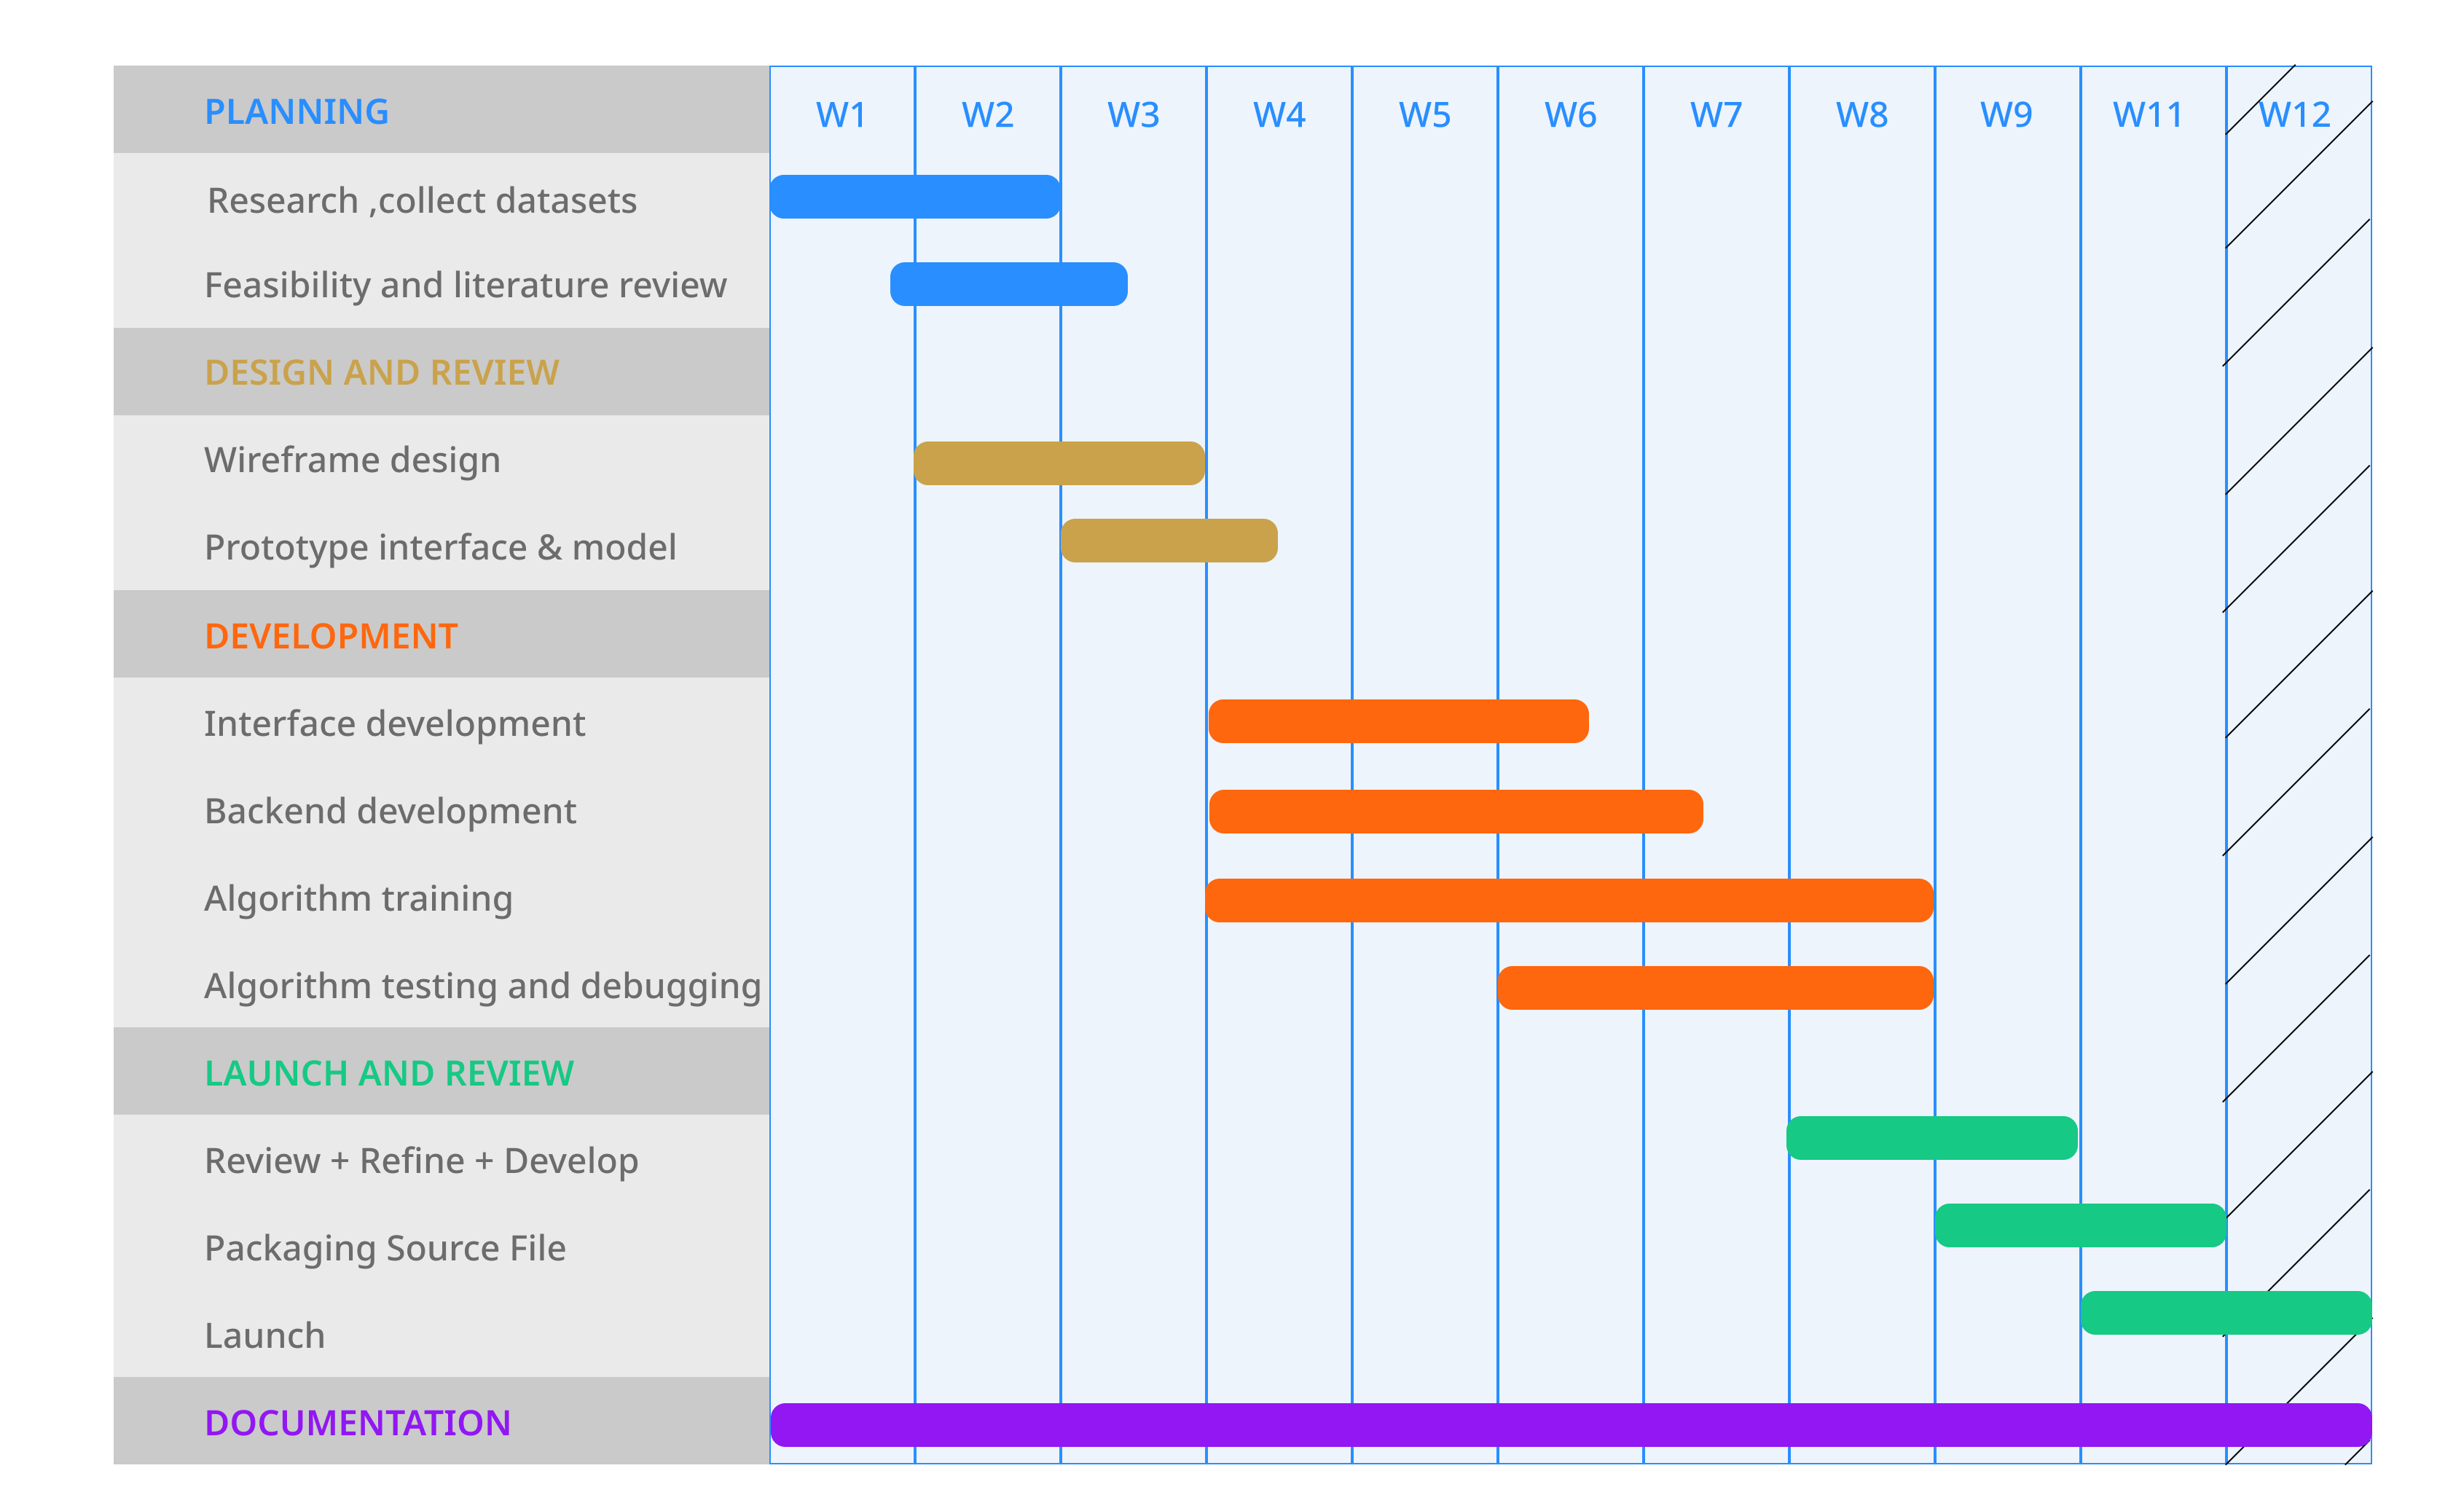
\includegraphics[width=150mm]{./img/gantt_chart.png}
    \caption{Gantt Chart}
\end{figure}